\documentclass[article]{jss}

%% -- LaTeX packages and custom commands ---------------------------------------

\usepackage{amsmath,amssymb,bm}
\usepackage{booktabs}

%% custom commands
\newcommand{\T}{\mathbf{T}}
\newcommand{\half}{\tfrac{1}{2}}

%% -- Article metainformation --------------------------------------------------

\author{Choonjoo Lee\\Korea National Defense University}
\Plainauthor{Choonjoo Lee}

\title{\pkg{sw2023}: Nonparametric Multiple-Output Stochastic Frontier
       Analysis in \proglang{Python} and \proglang{Stata}}
\Plaintitle{sw2023: Nonparametric Multiple-Output Stochastic Frontier
            Analysis in Python and Stata}
\Shorttitle{\pkg{sw2023}: Nonparametric Multiple-Output SFA}

\Abstract{
This paper presents \pkg{sw2023}, a \proglang{Python} package implementing the
nonparametric stochastic frontier model of \citet{SimarWilson2023} for
production technologies with multiple inputs and multiple outputs.
The estimator projects observations onto a directional distance function,
recovers the production frontier and individual efficiency scores via
local linear least squares (LLLS), and selects bandwidths by
leave-one-out cross-validation.
The package also provides a four-component panel extension decomposing
efficiency into transient and persistent components, bootstrap confidence
intervals for the frontier and individual efficiency scores,
asymptotic pointwise confidence bands based on the central limit theorem
and the delta method, and a wild bootstrap significance test for
inefficiency heterogeneity \citep{PSVKZ2024}.
A native \proglang{Stata} interface is also provided: \code{sw2023.ado}
implements the full estimation algorithm and bootstrap inference in
\proglang{Stata}~Mata without requiring a \proglang{Python} installation,
and the companion \code{sw2023test.ado} performs the PSVKZ wild bootstrap test.
A Monte Carlo study confirms that the implementation reproduces
\citet{SimarWilson2023} Table~F.1 across all five input--output
dimension combinations: integrated mean squared error (IMSE) ratios range
from 0.80 to 1.39 with median 1.01 (100 replications per cell).
}

\Keywords{stochastic frontier analysis, multiple outputs, nonparametric,
  efficiency, local linear regression, bootstrap, \proglang{Python},
  \proglang{Stata}}
\Plainkeywords{stochastic frontier analysis, multiple outputs,
  nonparametric, efficiency, local linear regression, bootstrap,
  Python, Stata}

\Address{
  Choonjoo Lee\\
  Department of AI and Robotics\\
  Korea National Defense University\\
  Nonsan, Republic of Korea\\
  E-mail: \email{bloom.rampike@gmail.com}
}

%%%%%%%%%%%%%%%%%%%%%%%%%%%%%%%%%%%%%%%%%%%%%%%%%%%%%%%%%%%%%%%%%%%%%%%%%%%%%%

\begin{document}


%% -- Introduction ------------------------------------------------------------

\section[Introduction]{Introduction}
\label{sec:intro}

Stochastic frontier analysis (SFA) is a principal tool for measuring
productive efficiency in economics \citep{SimarWilson2010}.  Most
implementations assume a parametric functional form for the frontier
(e.g., Cobb--Douglas or translog) and restrict the analysis to a single
output.  \citet{SimarWilson2023} propose a fully nonparametric framework
that handles \emph{multiple outputs} without imposing any functional form.
Their estimator is built on the directional output distance function and
employs local linear least squares (LLLS) to recover the conditional
moments of the composed error term.

Several related software packages exist, but none implements the
\citet{SimarWilson2023} estimator.
The \proglang{R} package \pkg{FEAR} \citep{Wilson2008} provides bootstrap
inference for DEA and free disposal hull estimators, but does not model
stochastic noise.
The \proglang{R} package \pkg{npsf} \citep{BadunenkoMozharovskyi2016}
implements parametric SFA (half-normal and truncated-normal inefficiency
distributions) for the \emph{single-output} case, alongside nonparametric
DEA-based efficiency analysis.
The \proglang{Python} package \pkg{pyStoNED} \citep{DaiFangLeeKuosmanen2024}
supports multiple-output frontier estimation via convex nonparametric least
squares (CNLS) combined with method-of-moments efficiency recovery
(the StoNED estimator of \citealt{KuosmanenJohnson2010}).
\pkg{pyStoNED} imposes global concavity and monotonicity constraints on the
frontier, relies on an external quadratic programming solver
(e.g., MOSEK or CPLEX), and does not provide bootstrap inference.
\pkg{sw2023}, by contrast, imposes no shape constraints, requires no external
solver, and offers a complete inference toolkit (bootstrap CIs, asymptotic
CIs via the delta method, and a wild bootstrap test for inefficiency
heterogeneity).
The \proglang{Ox} package \pkg{SFAMB} \citep{HoltkampBrummer2017} implements
various \emph{parametric} SFA models with panel extensions, but assumes a
Cobb--Douglas or translog functional form and a single output.

This paper fills this gap with \pkg{sw2023}, a \proglang{Python} package that
\begin{enumerate}
  \item implements the full \citet{SimarWilson2023} estimation algorithm
        (Steps~1--10) for arbitrary numbers of inputs $p$ and outputs $q$;
  \item extends the model to a four-component panel decomposition of
        transient and persistent inefficiency;
  \item provides pairs/cluster bootstrap confidence intervals with a
        corrected evaluation strategy (bootstrap sample fitted at original
        evaluation points);
  \item provides pointwise asymptotic confidence bands based on the CLT
        of \citet{SimarWilson2023} and the delta method;
  \item provides a wild bootstrap significance test for inefficiency
        heterogeneity following \citet{PSVKZ2024}.
\end{enumerate}

The remainder of the paper is organized as follows.
Section~\ref{sec:method} reviews the \citet{SimarWilson2023} model.
Section~\ref{sec:software} describes the package design and API.
Section~\ref{sec:inference} covers bootstrap and asymptotic inference.
Section~\ref{sec:mc} presents Monte Carlo validation against
\citet{SimarWilson2023} Table~F.1.
Section~\ref{sec:example} illustrates the package on simulated data.
Section~\ref{sec:summary} concludes.


%% -- Methodology -------------------------------------------------------------

\section[The Simar--Wilson (2023) estimator]{The Simar--Wilson (2023) Estimator}
\label{sec:method}

\subsection{Model and identification}
\label{sec:model}

Let $\mathbf{x} \in \mathbb{R}^p_+$ be an input vector and
$\mathbf{y} \in \mathbb{R}^q_+$ be an output vector.
The production technology is characterized by the output set
$\mathcal{P}(\mathbf{x}) = \{\mathbf{y} : (\mathbf{x},\mathbf{y})
\text{ is feasible}\}$.  Following \citet{SimarWilson2023}, this paper adopts
the \emph{directional output distance function}
%
\begin{equation}
  D_O(\mathbf{x},\mathbf{y};\mathbf{d})
  = \sup\!\left\{\beta \geq 0 : \mathbf{y}+\beta\mathbf{d}_y
                                \in \mathcal{P}(\mathbf{x}-\beta\mathbf{d}_x)
               \right\},
\end{equation}
%
where $\mathbf{d} = (\mathbf{d}_x,\mathbf{d}_y) \in \mathbb{R}^{p+q}$ is
a direction vector normalized to $\|\mathbf{d}\|=1$.

The observed data follow the stochastic model
%
\begin{equation}
  U_i = \varphi(\mathbf{Z}_i) + \|\mathbf{d}\|\,(\varepsilon_i - \eta_i),
  \label{eq:model}
\end{equation}
%
where $U_i = D_O(\mathbf{x}_i,\mathbf{y}_i;\mathbf{d})$ is the observed
directional distance, $\mathbf{Z}_i \in \mathbb{R}^{p+q-1}$ is the
vector of coordinates orthogonal to $\mathbf{d}$, $\varphi(\cdot)$ is the
unknown frontier function, $\varepsilon_i \sim N(0,\sigma_\varepsilon^2(\mathbf{Z}_i))$
is symmetric noise, and $\eta_i \sim |N(0,\sigma_\eta^2(\mathbf{Z}_i))|$
is the nonnegative inefficiency term.

\subsection{Estimation algorithm}
\label{sec:algo}

The estimation proceeds in ten steps \citep{SimarWilson2023}.

\textbf{Step~1.} Choose direction vector $\mathbf{d}$.  Typical choices
are the component-wise sample mean or median of $(X,Y)$.

\textbf{Steps~2--3.} Rotate the data: compute $U_i$ (projection along
$\mathbf{d}$) and $\mathbf{Z}_i$ (projection onto the orthogonal
complement of $\mathbf{d}$).

Figure~\ref{fig:rotation} illustrates the rotation for $p = q = 1$.
Panel~(A) shows observations in the original input--output space
with the direction vector $\mathbf{d}$ (red) and its orthogonal
complement $\mathbf{v}$ (gray).  Colored arrows indicate the
directional projection of each highlighted firm onto the frontier.
Panel~(B) shows the same data after applying $R_{\mathbf{d}}$:
the frontier $\varphi(\mathbf{Z})$ becomes a regression function
of~$Z$, the vertical gap $\eta_i + \varepsilon_i$ is the composite
error, and the LLLS target $\hat{r}_1(Z) = \varphi(Z)-\mu_\eta$ is
shifted below the frontier by $\mu_\eta = \sqrt{2/\pi}\,\hat\sigma_\eta$.
Panel~(C) contrasts the data-driven direction $\mathbf{d}$ of
SW(2023) against the fixed output-direction of traditional SFA
($\mathbf{d}=(0,1)$), which fails when $q>1$.

\begin{figure}[t!]
\centering
\includegraphics[width=\textwidth]{fig_rotation}
\caption{\label{fig:rotation}%
  SW(2023) direction-vector rotation for $p=q=1$ (DGP: quarter-circle
  production frontier, $n=70$, $\sigma_\eta=0.09$).
  \textbf{(A)}~Input--output space: the direction vector
  $\mathbf{d} = (-\bar{X}, \bar{Y})/\|\cdot\|$ (red arrow) and its
  orthogonal complement $\mathbf{v}$ (gray) define the rotation
  $R_{\mathbf{d}}$.  Colored arrows show the directional
  projection $U_i = \mathbf{d}^\top\mathbf{W}_i$ of four selected
  observations (circles) onto the frontier (diamonds).
  \textbf{(B)}~Rotated space $(Z,U)$: the frontier $\varphi(Z)$
  (solid) becomes a standard regression function; the LLLS
  conditional mean $\hat{r}_1(Z) = \varphi(Z)-\mu_\eta$ (dashed)
  lies below it by the inefficiency bias $\mu_\eta$.
  \textbf{(C)}~Directional projection: SW(2023) uses a
  data-driven $\mathbf{d}$ (red) that generalizes to any $(p,q)$,
  whereas traditional output-oriented SFA uses $\mathbf{d}=(0,1)$
  (orange), which requires $q=1$.
}
\end{figure}

\textbf{Steps~4--6.} Estimate conditional moments by LLLS \citep{FanGijbels1996}:
%
\begin{align}
  \hat{r}_1(\mathbf{z}) &= \hat{E}[U \mid \mathbf{Z}=\mathbf{z}], \\
  \hat{r}_2(\mathbf{z}) &= \hat{E}[\hat{\varepsilon}^2 \mid \mathbf{Z}=\mathbf{z}], \\
  \hat{r}_3(\mathbf{z}) &= \hat{E}[\hat{\varepsilon}^3 \mid \mathbf{Z}=\mathbf{z}],
\end{align}
%
where $\hat{\varepsilon}_i = U_i - \hat{r}_1(\mathbf{Z}_i)$.
Bandwidths are selected by leave-one-out cross-validation (LOO-CV)
separately for each regression.

\textbf{Step~7.} Estimate $\hat{\sigma}_\eta(\mathbf{z})$ from
$\hat{r}_3(\mathbf{z})$:
%
\begin{equation}
  \hat{\sigma}_\eta(\mathbf{z}) = \max\!\left\{0,
    \left(\frac{-\hat{r}_3(\mathbf{z})}{a_3^+}\right)^{1/3}\right\}, \quad
  a_3^+ = \frac{4-\pi}{\pi}\sqrt{\frac{2}{\pi}} \approx 0.2177.
\end{equation}
%
When $\hat{r}_3(\mathbf{z})>0$ (the ``wrong skewness'' case), the HMS
estimator \citep{HafnerMannerSimar2018} uses
$\hat{\sigma}_\eta(\mathbf{z}) = (r_3/a_3^-)^{1/3}$
with $a_3^- \approx 0.01674$.

\textbf{Step~8.} Estimate $\hat{\sigma}_\varepsilon(\mathbf{z})$:
%
\begin{equation}
  \hat{\sigma}_\varepsilon^2(\mathbf{z})
  = \hat{r}_2(\mathbf{z}) - \frac{\pi-2}{\pi}\hat{\sigma}_\eta^2(\mathbf{z}).
\end{equation}

\textbf{Step~9.} Estimate the frontier:
%
\begin{equation}
  \hat{\varphi}(\mathbf{z}) = \hat{r}_1(\mathbf{z})
  + \|\mathbf{d}\|\sqrt{\tfrac{2}{\pi}}\,\hat{\sigma}_\eta(\mathbf{z}).
  \label{eq:frontier}
\end{equation}

\textbf{Step~10.} Estimate individual efficiency via JLMS
\citep{JondrowEtAl1982}:
%
\begin{equation}
  \hat{\eta}_i = E[\eta_i \mid \hat{\xi}_i, \mathbf{Z}_i], \quad
  \widehat{\mathrm{eff}}_i = \exp(-\hat{\eta}_i) \in (0,1].
\end{equation}

\subsection{Bandwidth selection}
\label{sec:bandwidth}

The LOO-CV bandwidth minimizes
$\mathrm{CV}(h) = n^{-1}\sum_i (U_i - \hat{U}_{-i})^2$,
where $\hat{U}_{-i}$ is the leave-one-out fitted value computed via
the hat-matrix trick
$\hat{U}_{-i} = (\hat{U}_i - h_{ii}U_i)/(1-h_{ii})$
with $h_{ii} = [(X^\top W_i X)^{-1}]_{00}$
\citep{FanGijbels1996}.

A scalar multiplier $c > 0$ is optimized so that
$h_k = c \cdot h_k^{\mathrm{ref}}$ with
$h_k^{\mathrm{ref}} = \hat{\sigma}_k n^{-1/(d+4)}$.
The lower bound for $c$ is determined adaptively by requiring the
average effective sample size
$n_{\mathrm{eff}}(c) = n^{-1}\sum_i\sum_j K_c(\mathbf{Z}_i,\mathbf{Z}_j)
\geq k_{\min}$
where $k_{\min} = \max(5, 2(d+2))$ and $d = p+q-1$.
The full product-kernel variant (\code{bandwidth\_method='loocv'})
optimizes each $h_k$ independently via coordinate descent,
consistent with the Banking Application in \citet{SimarWilson2023}
Table~G.2.
The scalar variant (\code{bandwidth\_method='loocv\_scalar'})
constrains all $h_k = c \cdot h_k^{\mathrm{ref}}$ and is retained
for backward compatibility.

Figure~\ref{fig:bw_comparison} illustrates the practical effect of
bandwidth choice on a synthetic single-input single-output dataset
($p=q=1$, $n=300$).
The Silverman rule selects a bandwidth that is too small, producing
an over-fitted frontier with spurious oscillations.
Both LOO-CV variants select a larger, better-smoothed bandwidth and
yield nearly identical efficiency distributions.
For $d=1$ the scalar and product optimisations coincide exactly, as
expected.

\begin{figure}[t!]
\centering
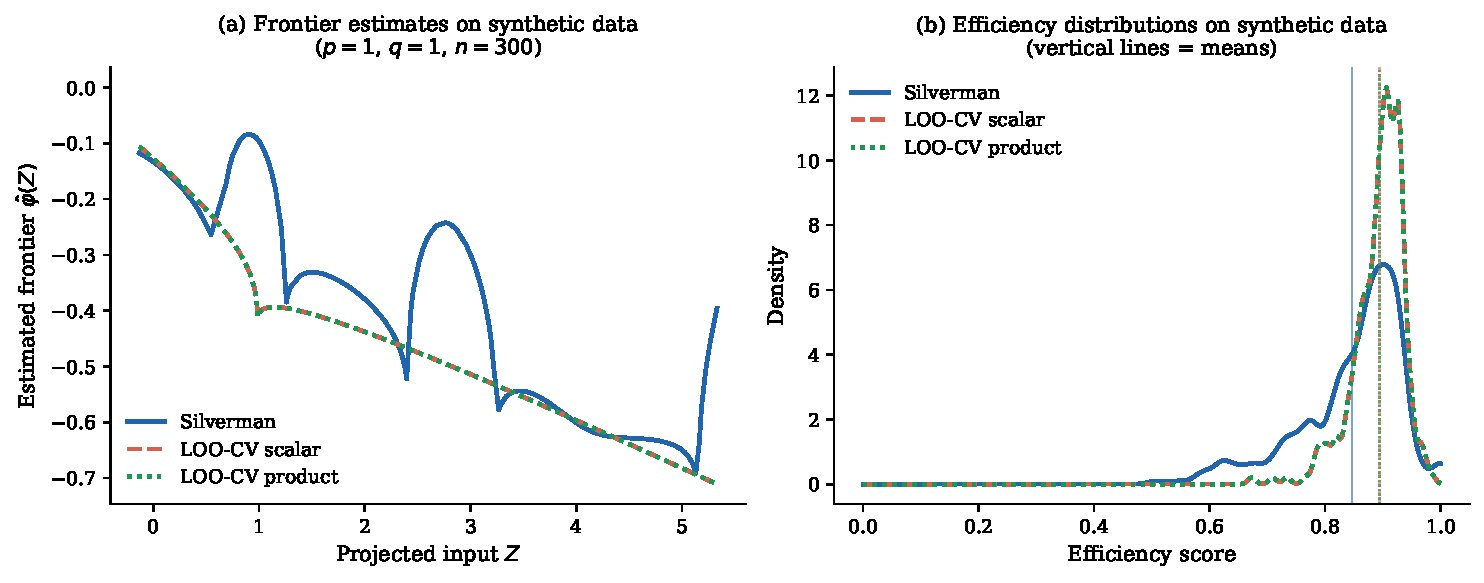
\includegraphics[width=\textwidth]{fig_synthetic_comparison}
\caption{\label{fig:bw_comparison}%
  Effect of bandwidth method on frontier estimation ($p=q=1$, $n=300$,
  true frontier $\varphi(Z)=2\ln Z$, $\sigma_v=0.20$, $\sigma_u=0.30$).
  \emph{Left}: estimated frontier $\hat\varphi(Z)$ versus projected
  input $Z$.  The Silverman rule selects an excessively small bandwidth,
  causing over-fitting (oscillations); both LOO-CV methods select
  a larger bandwidth and produce smooth estimates.
  For $d=p+q-1=1$ the scalar and product LOO-CV optimisations are
  equivalent and their curves coincide.
  \emph{Right}: kernel density estimates of efficiency scores.
  Silverman inflates efficiency estimates due to over-fitting;
  LOO-CV gives a more concentrated distribution near the true mean.}
\end{figure}


%% -- Software ----------------------------------------------------------------

\section[Software description]{Software Description}
\label{sec:software}

\subsection{Package structure}
\label{sec:structure}

\pkg{sw2023} is organized into four sub-packages:
%
\begin{Code}
sw2023/
  __init__.py            # public API
  core/
    model.py             # SW2023Model class
    frontier.py          # LLLS, hat-matrix, leverages
    decompose.py         # sigma_eta, sigma_eps, JLMS
    bandwidth.py         # LOO-CV, Silverman rule
    bootstrap.py         # pairs bootstrap, wild bootstrap
    transform.py         # direction vector, rotation
    preprocess.py        # log transform, standardize
  panel/
    four_component.py    # PanelSW2023 class
  stata/
    sw2023_stata.py        # Stata 16.1+ Python script interface
    sw2023.ado             # native Stata/Mata implementation
    sw2023_example.do      # Python-bridge example do-file
    sw2023_native_example.do  # ado-file example do-file
  tests/
    test_model.py        # pytest (13 tests)
    monte_carlo.py       # Monte Carlo validation
\end{Code}

\subsection{Main classes and functions}
\label{sec:api}

The public API is accessible directly from \code{import sw2023}.

\code{SW2023Model(X, Y, direction, method, bandwidth\_method)} is the
main cross-sectional model class.  After calling \code{model.fit()},
results are stored as attributes: \code{phi\_hat\_} (frontier values),
\code{efficiency\_} (JLMS efficiency scores),
\code{sigma\_eta\_} (inefficiency standard deviation), and
\code{r1\_}, \code{r2\_}, \code{r3\_} (conditional moment estimates).

\code{PanelSW2023(X, Y, firm\_id, time\_id)} extends the model to
panel data.  Fitted attributes include \code{eff\_transient\_} and
\code{eff\_persistent\_}.

\code{bootstrap\_sw(X, Y, B, alpha)} returns pairs bootstrap confidence
intervals for the frontier, individual efficiency, and
$\hat{\sigma}_\eta$.  \code{bootstrap\_panel()} provides the cluster
bootstrap analog for panel data.

\code{test\_r3\_significance(X, Y, B)} implements the wild bootstrap test
for inefficiency heterogeneity of \citet{PSVKZ2024}.

\code{bandwidth\_loocv(Z, y)} performs standalone LOO-CV bandwidth
selection.

\subsection{Installation}
\label{sec:install}

\pkg{sw2023} (version~0.3.0) requires \proglang{Python}~$\geq 3.8$ and
depends on \pkg{numpy} \citep{HarrisEtAl2020},
\pkg{scipy} \citep{VirtanenEtAl2020}, and \pkg{pandas} \citep{McKinney2010}.
It is distributed under the GNU General Public License (GPL-3.0-or-later) and is available from the
Python Package Index (PyPI) at \url{https://pypi.org/project/sw2023/}:
%
\begin{Code}
pip install sw2023
\end{Code}
%
An optional visualization dependency (\pkg{matplotlib}) is installed with:
%
\begin{Code}
pip install sw2023[viz]
\end{Code}
%
All results are fully reproducible via the standalone script
\code{replication.py} included with the submission materials.
The random seed is fixed (\code{np.random.seed(42)}); Sections~6.1--6.2
reproduce exactly, while bootstrap results (Sections~6.3--6.4) are
subject to Monte Carlo variation.


\subsection{Stata interface}
\label{sec:stata}

\pkg{sw2023} provides two complementary \proglang{Stata} interfaces:
a \proglang{Python}-script bridge and a self-contained native ado-file,
both located in the \code{stata/} sub-directory.

\paragraph{Python-script bridge.}
For users with \proglang{Stata}~16.1 or later and \proglang{Python}~3.8+
configured via \code{python set exec}, the script \code{sw2023\_stata.py}
is invoked through \proglang{Stata}'s \code{python~script} command.
A pipe-delimited argument string specifies inputs, outputs, and options:
%
\begin{CodeChunk}
\begin{CodeInput}
Stata> python set exec "/usr/local/bin/python3"
Stata> local sw_args "x1 x2 | y1 y2 | method=HMS"
Stata> python script "sw2023/stata/sw2023_stata.py"
\end{CodeInput}
\begin{CodeOutput}
[SW2023] 2-component cross-sectional model
  Inputs (2): x1 x2  |  Outputs (2): y1 y2  |  Method: HMS
  Mean efficiency: 0.4563
  New variables: sw_efficiency, sw_sigma_eta, sw_r1, sw_r3
  Done.
\end{CodeOutput}
\end{CodeChunk}
%
The four-component panel model is invoked by passing \code{args("panel")}
with \code{firm=} and \code{time=} identifiers.

\paragraph{Native ado-file.}
\begin{sloppypar}
For \proglang{Stata}-only workflows that do not require a
\proglang{Python} installation, \code{sw2023.ado} implements the
complete SW(2023) ten-step algorithm in \proglang{Stata}~Mata,
including pairs bootstrap CIs \citep{SimarWilson2023} and the
PSVKZ wild bootstrap significance test \citep{PSVKZ2024}.%
\footnote{The companion command \code{sw2023test} performs the wild
  bootstrap test for heterogeneous inefficiency and is defined in
  the self-contained \code{sw2023test.ado}.}
After copying both ado-files to a folder on \code{adopath},
the commands follow standard \proglang{Stata} conventions:
\end{sloppypar}
%
\begin{CodeChunk}
\begin{CodeInput}
. sw2023 y1 y2, inputs(x1 x2) direction(mean) method(hms)  ///
>               bandwidth(silverman) bootstrap(199) level(95)
\end{CodeInput}
\begin{CodeOutput}
[sw2023] Nonparametric Multiple-Output SFA
  Outputs  : y1 y2   Inputs : x1 x2   N : 200   p/q : 2 / 2
  direction: mean    method : hms      bandwidth: silverman
  bootstrap: B=199, 95% CI

  Mean efficiency : 0.4571
  Std  efficiency : 0.2318
  Mean sigma_eta  : 1.2011
  Mean eff CI     : [0.3812, 0.5344]  (95%)

[sw2023] Done.
\end{CodeOutput}
\end{CodeChunk}
%
\begin{CodeChunk}
\begin{CodeInput}
. sw2023test y1 y2, inputs(x1 x2) reps(299)
\end{CodeInput}
\begin{CodeOutput}
[sw2023test] Wild Bootstrap Significance Test
  H0: E(eps^3 | Z) = const  (homogeneous inefficiency)
  H1: E(eps^3 | Z) != const (heterogeneous)
  N: 200   Reps: 299

  Test statistic T :   0.039742
  Bootstrap p-value:   0.8696
  => Fail to reject H0: homogeneous inefficiency

[sw2023test] Done.
\end{CodeOutput}
\end{CodeChunk}
%
\begin{sloppypar}
The \code{sw2023} command accepts \code{direction(mean|median)},
\code{method(hms|svkz)}, \code{bandwidth(silverman|loocv)},
\code{bootstrap($B$)} for the SW pairs bootstrap,
\code{level(\#)} for CI coverage (default~95), and
\code{generate()} for the output prefix (default \code{sw\_}).
Point-estimate results are stored in \code{sw\_efficiency},
\code{sw\_phi\_hat}, \code{sw\_sigma\_eta}, \code{sw\_sigma\_eps},
\code{sw\_r1}, \code{sw\_r2}, \code{sw\_r3}
(the three LLLS conditional-moment estimates $\hat r_k(Z_i)$).
With \code{bootstrap()}, six CI variables are added:
\code{sw\_eff\_lo}/\code{sw\_eff\_hi},
\code{sw\_phi\_lo}/\code{sw\_phi\_hi}, and
\code{sw\_seta\_lo}/\code{sw\_seta\_hi}.
The \code{sw2023test} command returns
\code{r(statistic)} and \code{r(p\_value)}.
\end{sloppypar}

The SW pairs bootstrap \citep{SimarWilson2023} resamples $(X_i, Y_i)$
with replacement, rotates the bootstrap sample using the \emph{fixed}
direction vector $\hat{\mathbf{d}}$ from the original fit,
re-estimates $\hat{r}_k^*(Z)$ on the bootstrap data,
and evaluates at the original $Z_i$ points.
The PSVKZ wild bootstrap \citep{PSVKZ2024} applies Rademacher
multipliers ($V_i \in \{-1,+1\}$) to the centred residuals
$\hat\eta_i^c = \hat\varepsilon_i^3 - \hat r_3(Z_i) -
\overline{(\hat\varepsilon^3 - \hat r_3)}$
and re-estimates $\hat r_3^*$ on
$\hat\varepsilon_i^{3*} = \hat r_3(Z_i) + \hat\eta_i^c\,V_i$.
On the simulation data set ($n=200$, $p=q=2$), point estimation
completes in under one second; $B=199$ bootstrap replications
take approximately thirty seconds.
Observations with any missing input or output are excluded
automatically, and a worked example do-file
(\code{sw2023\_native\_example.do}) is included in the
\code{stata/} sub-directory.


\subsection{Comparison with related software}
\label{sec:comparison}

Table~\ref{tab:comparison} compares \pkg{sw2023} against the most closely
related packages along seven dimensions that matter for applied researchers.

\begin{table}[t!]
\centering
\caption{\label{tab:comparison}%
  Feature comparison of nonparametric/semiparametric frontier software:
  \pkg{sw2023} (this paper), \pkg{pyStoNED} \citep{DaiFangLeeKuosmanen2024},
  \pkg{npsf} \citep{BadunenkoMozharovskyi2016}, and
  \pkg{FEAR} \citep{Wilson2008}.
  ``Shape constr.''\ = global concavity/monotonicity imposed on frontier.
  ``Bootstrap'' = bootstrap CIs or hypothesis tests available.}
\smallskip
\small
\begin{tabular}{lcccc}
\toprule
Feature               & \pkg{sw2023} & \pkg{pyStoNED} & \pkg{npsf} & \pkg{FEAR} \\
\midrule
Language              & Python & Python & R      & R \\
Multiple outputs      & Yes    & Yes    & No     & No \\
Stochastic noise      & Yes    & Yes    & Yes    & No \\
Frontier estimator    & LLLS   & CNLS   & MLE    & DEA/FDH \\
Shape constr.\        & None   & Concave + monotone & None & Monotone \\
External solver       & No     & Yes (QP) & No   & No \\
Bootstrap inference   & Yes    & No     & Yes    & Yes \\
Panel (4-component)   & Yes    & No     & No     & No \\
\proglang{Stata} interface & Yes & No  & No     & No \\
\bottomrule
\end{tabular}
\end{table}

The most salient methodological difference between \pkg{sw2023} and
\pkg{pyStoNED} is the treatment of the frontier shape.
CNLS imposes concavity and monotonicity globally via a system of $O(n^2)$
inequality constraints solved by quadratic programming; this guarantees
theoretically consistent shape but requires a commercial or academic
solver licence (MOSEK, CPLEX, or KNITRO) and limits scalability ---
the \pkg{pyStoNED} documentation recommends a remote NEOS server for
$n > 500$.
\pkg{sw2023} uses LLLS without shape restrictions, requiring only
\proglang{NumPy} and \proglang{SciPy}, and runs efficiently on samples
of several thousand observations on a standard laptop.
Statistically, CNLS provides a deterministic envelope from which
efficiency is extracted by method of moments \citep{KuosmanenJohnson2010},
whereas \pkg{sw2023} embeds efficiency directly in the LLLS regression
residuals and recovers the frontier through the CLT-based decomposition
of \citet{SimarWilson2023}; this yields the bootstrap and asymptotic
inference machinery described in Section~\ref{sec:inference}.

\paragraph{Cross-application to the Finnish electricity dataset.}
To facilitate direct comparison, we apply \pkg{sw2023} to the Finnish
electricity distribution dataset used throughout the \pkg{pyStoNED}
paper \citep{DaiFangLeeKuosmanen2024}: 89~firms with two inputs
(OPEX, CAPEX) and three outputs (energy delivered, network length,
number of customers).
With Silverman bandwidth selection, \pkg{sw2023} estimates a mean
production efficiency of $\hat\mu_{\mathrm{eff}} = 0.870$ (median
$0.889$, standard deviation $0.091$), ranging from $0.595$ to $0.999$.
The HMS wrong-skewness correction is triggered for 59.6\% of
observations --- a moderately noisy sample for which the automatic
correction prevents sign reversals in $\hat\sigma_\eta$.
With per-dimension product-kernel LOO-CV (\code{bandwidth\_method='loocv'}),
mean efficiency falls to $0.809$ (median $0.825$, standard deviation
$0.125$), reflecting the more flexible local bandwidth adaptation.
Because \pkg{pyStoNED} models the same data as a \emph{cost} frontier
(inputs = service outputs, output = total cost), its efficiency scores
are cost-efficiency measures and are not numerically comparable to the
production-efficiency scores above; the datasets and variable roles
are, however, identical.

\paragraph{Practical guidance.}
Researchers should prefer \pkg{pyStoNED} when a production or cost
function is \emph{a priori} known to be concave (or convex) and
monotone, and when a suitable QP solver is available; the shape
constraints provide efficiency gains under correct specification.
\pkg{sw2023} is the natural choice when shape constraints are
untestable or potentially misspecified, when bootstrap inference or
panel decomposition is required, when large samples rule out $O(n^2)$
QP, or when a pure-Python deployment without external solvers is
needed.  The two packages are therefore largely complementary rather
than competing.


%% -- Inference ---------------------------------------------------------------

\section[Statistical inference]{Statistical Inference}
\label{sec:inference}

\subsection{Bootstrap confidence intervals}
\label{sec:bootstrap}

The pairs bootstrap proceeds as follows for each replication
$b = 1,\ldots,B$:
\begin{enumerate}
  \item Draw $n$ indices $\{i_1,\ldots,i_n\}$ with replacement from
        $\{1,\ldots,n\}$.
  \item Apply the \emph{original} preprocessing parameters and direction
        vector $\hat{\mathbf{d}}$ to the resampled data.
  \item Fit the LLLS regressions on the bootstrap sample
        $(\mathbf{Z}^*_b, U^*_b)$ with bandwidth $h^*_b$.
  \item Evaluate the bootstrap frontier at the \emph{original} evaluation
        points $\mathbf{Z}_i$:
        $\hat{\varphi}^*_b(\mathbf{Z}_i) = \hat{r}^*_{1,b}(\mathbf{Z}_i)
         + \|\hat{\mathbf{d}}\|\sqrt{2/\pi}\,\hat{\sigma}^*_{\eta,b}(\mathbf{Z}_i)$.
  \item Compute individual efficiency at original $U_i$:
        $\widehat{\mathrm{eff}}^*_{b,i} = \exp(-\hat{\eta}^*_{b,i})$.
\end{enumerate}
Step~4 uses an internal \code{eval\_points} argument so that bootstrap fits
are always evaluated at the original $Z$ grid.  This corrects the common
error of comparing bootstrap fitted values at resampled points to the
original point estimates.

The $100(1-\alpha)\%$ confidence interval (CI) for
$\hat{\varphi}(\mathbf{Z}_i)$ is
%
\begin{equation}
  \left[\hat{Q}_{\alpha/2}\!\left(\hat{\varphi}^*_b(\mathbf{Z}_i)\right),\;
         \hat{Q}_{1-\alpha/2}\!\left(\hat{\varphi}^*_b(\mathbf{Z}_i)\right)\right].
\end{equation}

\subsection{Asymptotic confidence intervals}
\label{sec:asymptotic}

By \citet{SimarWilson2023} Eq.~(3.8) and standard local linear regression
theory \citep{FanGijbels1996}, at an interior point $\mathbf{z}$:
%
\begin{equation}
  \bigl(nh^{d-1}\bigr)^{1/2}
  \bigl(\hat{r}_j(\mathbf{z}) - r_j(\mathbf{z})\bigr)
  \xrightarrow{d} N\!\bigl(0, s^2_j(\mathbf{z})\bigr),
  \quad j \in \{1,2,3\},
\end{equation}
%
where $d = p+q-1$.  The asymptotic variance is estimated via
%
\begin{equation}
  \widehat{\mathrm{AVar}}\bigl(\hat{r}_j(\mathbf{z}_i)\bigr)
  \approx h^{(j)}_{ii} \cdot \hat{\sigma}^2_j(\mathbf{z}_i),
\end{equation}
%
with hat-matrix leverage
$h^{(j)}_{ii} = [(X^\top W_j X)^{-1}]_{00}$
and local conditional variance
$\hat{\sigma}^2_j(\mathbf{z}_i)$ estimated by an auxiliary LLLS
regression of $(\hat{\varepsilon}^j - \hat{r}_j)^2$ on $\mathbf{Z}$.

The asymptotic CI for $\hat{\varphi}(\mathbf{z}_i)$ follows from the
delta method:
%
\begin{equation}
  \widehat{\mathrm{SE}}\bigl(\hat{\varphi}(\mathbf{z}_i)\bigr)^2
  \approx
  h^{(1)}_{ii}\,\hat{r}_2(\mathbf{z}_i) +
  \left(\frac{\partial\varphi}{\partial r_3}\right)^2
  h^{(3)}_{ii}\,\hat{\sigma}^2_3(\mathbf{z}_i),
\end{equation}
%
where
$\partial\varphi/\partial r_3
 = -\|\hat{\mathbf{d}}\|\sqrt{2/\pi}\,
   \bigl(3\,a_3^+\,\hat{\sigma}^2_\eta(\mathbf{z}_i)\bigr)^{-1}$
for $\hat{r}_3(\mathbf{z}_i)\leq 0$.

\subsection{Wild bootstrap significance test}
\label{sec:wildbootstrap}

Following \citet{PSVKZ2024} Section~3.1, this paper tests
$H_0: E(\varepsilon^3 \mid \mathbf{Z}) = \mathrm{const}$
against heterogeneous inefficiency using the statistic
%
\begin{equation}
  T = \frac{\mathrm{Var}\bigl(\hat{r}_3(\mathbf{Z})\bigr)}
           {\mathrm{Var}(\hat{\varepsilon}^3)}.
\end{equation}
%
The wild bootstrap uses Rademacher perturbations
$\hat{\varepsilon}^{3,*}_i = \hat{r}_3(\mathbf{Z}_i) + \eta^c_i V_i$,
$V_i \sim \{-1,+1\}$ with equal probability, where
$\eta^c_i = (\hat{\varepsilon}^3_i - \hat{r}_3(\mathbf{Z}_i))
             - n^{-1}\sum_j(\cdot)$
are the centered residuals.


%% -- Monte Carlo -------------------------------------------------------------

\section[Monte Carlo validation]{Monte Carlo Validation}
\label{sec:mc}

This paper replicates the Monte Carlo study of \citet{SimarWilson2023}
Appendix~F.  The data-generating process uses the sphere construction of
\citet{Marsaglia1972}: observations are drawn uniformly from a unit
sphere of dimension $p+q$, giving the frontier as the sphere surface and
the directional distance $U^*_i$ as the true target.

The inefficiency is $\eta_i \sim |N(0,0.5^2)|$ and the noise is
$\varepsilon_i \sim N(0, \rho^2 \sigma_\eta^2)$
with $\rho \in \{0, 0.5, 1.0, 2.0\}$.

The integrated mean squared error (IMSE) is
%
\begin{equation}
  \widehat{\mathrm{IMSE}} = \frac{1}{n}\sum_{i=1}^n
  \bigl(\hat{\varphi}(\mathbf{Z}_i) - U^*_i\bigr)^2.
\end{equation}

Table~\ref{tab:imse} reports the ratio of \pkg{sw2023}'s average IMSE
over 100 Monte Carlo replications to \citet{SimarWilson2023} Table~F.1
for all five $(p,q)$ combinations.

\begin{table}[t!]
\centering
\caption{\label{tab:imse} IMSE ratios: \pkg{sw2023} / SW(2023) Table~F.1.
         Ratios based on 100 Monte Carlo replications per cell.
         A ratio of 1.00 indicates exact match; ``---'' indicates
         no corresponding entry in Table~F.1 ($\rho > 0$, $n = 800$ for
         $(1,1)$ and $(2,2)$).  For $(1,2)$, $(2,3)$, and $(3,3)$,
         Table~F.1 reports only $\rho = 0$, so only one row is shown.
         For each of the three local-linear regressions
         ($\hat{r}_1$, $\hat{r}_2$, $\hat{r}_3$), bandwidths are selected
         independently via LOO-CV using a product kernel with per-dimension
         bandwidths $(h_1,\ldots,h_d)$, consistent with \citet{SimarWilson2023}
         Table~G.2.  Optimisation uses coordinate descent over $h_k$
         (Algorithm: \code{bandwidth\_loocv\_product}).}
\begin{tabular}{llrrrr}
\toprule
$(p,q)$ & $\rho$ & $n=100$ & $n=200$ & $n=400$ & $n=800$ \\
\midrule
(1,1) & 0.0 & 0.94 & 1.17 & 1.02 & 1.06 \\
(1,1) & 0.5 & 0.88 & 0.85 & 1.08 & --- \\
(1,1) & 1.0 & 0.98 & 0.86 & 0.97 & --- \\
(1,1) & 2.0 & 0.99 & 0.80 & 0.82 & --- \\
\midrule
(1,2) & 0.0 & 1.12 & 1.00 & 1.08 & 0.88 \\
\midrule
(2,2) & 0.0 & 0.95 & 1.14 & 1.29 & 1.28 \\
(2,2) & 0.5 & 0.96 & 1.13 & 1.29 & --- \\
(2,2) & 1.0 & 0.92 & 1.11 & 1.25 & --- \\
(2,2) & 2.0 & 0.94 & 1.02 & 1.05 & --- \\
\midrule
(2,3) & 0.0 & 0.93 & 1.02 & 1.14 & 1.39 \\
\midrule
(3,3) & 0.0 & 0.93 & 0.88 & 0.98 & 1.24 \\
\bottomrule
\end{tabular}
\end{table}

All ratios lie between 0.80 and 1.39, with an overall median of 1.01.
The $(2,2)$ and larger cases show ratios up to 1.39 for $n=800$,
consistent with the curse of dimensionality ($d = p+q-1 \geq 3$) and the
slower convergence rate $n^{2/(d+4)}$.

Table~\ref{tab:bw_compare} compares the scalar and per-dimension
product-kernel LOO-CV variants for $(p,q) \in \{(1,1),(2,2)\}$.
For $(p,q)=(1,1)$ the two methods are theoretically identical ($d=1$)
and the ratios agree to within Monte Carlo noise throughout.
For $(p,q)=(2,2)$ ($d=3$) the product kernel yields substantially
higher IMSE ratios at small $n$: the ratio reaches 2.10 at $n=100$,
$\rho=0.5$, more than double the scalar result of 0.96.
This deterioration diminishes as $n$ grows --- at $n=400$ the
difference is at most 0.16 --- consistent with the larger variance
of a three-dimensional coordinate-descent search in small samples.
Practitioners should therefore prefer \code{loocv\_scalar} when
$n \lesssim 200$ and $d \geq 3$, and reserve \code{loocv} (product)
for larger samples where per-dimension adaptation is beneficial.

\begin{table}[t!]
\centering
\caption{\label{tab:bw_compare}%
  IMSE ratios: scalar LOO-CV / product LOO-CV, for $(p,q)=(1,1)$
  ($d=1$) and $(p,q)=(2,2)$ ($d=3$).
  Each cell shows \textit{scalar\,/\,product}; ``---'' = no SW(2023)
  reference value available.
  For $d=1$ the two methods are equivalent by construction.
  For $d=3$ the product kernel inflates IMSE at small $n$ due to
  high-variance bandwidth search; the gap narrows as $n$ increases.}
\smallskip\small
\begin{tabular}{llrrrr}
\toprule
$(p,q)$ & $\rho$ & $n=100$ & $n=200$ & $n=400$ & $n=800$ \\
\midrule
\multicolumn{6}{l}{\textit{$d=1$: scalar $\equiv$ product}} \\
(1,1) & 0.0 & 0.94 / 0.94 & 1.17 / 1.15 & 1.02 / 1.02 & 1.06 / 1.06 \\
(1,1) & 0.5 & 0.88 / 0.88 & 0.85 / 0.85 & 1.08 / 1.10 & --- \\
(1,1) & 1.0 & 0.98 / 0.97 & 0.86 / 0.77 & 0.97 / 1.08 & --- \\
(1,1) & 2.0 & 0.99 / 0.99 & 0.80 / 0.78 & 0.82 / 0.82 & --- \\
\midrule
\multicolumn{6}{l}{\textit{$d=3$: product inflates IMSE at small $n$}} \\
(2,2) & 0.0 & 0.95 / \textbf{2.03} & 1.14 / 1.41 & 1.29 / 1.45 & 1.28 / 1.23 \\
(2,2) & 0.5 & 0.96 / \textbf{2.10} & 1.13 / 1.52 & 1.29 / 1.29 & --- \\
(2,2) & 1.0 & 0.92 / \textbf{1.67} & 1.11 / 1.51 & 1.25 / 1.24 & --- \\
(2,2) & 2.0 & 0.94 / 1.24 & 1.02 / 1.18 & 1.05 / 1.12 & --- \\
\bottomrule
\end{tabular}
\end{table}


%% -- Example -----------------------------------------------------------------

\section[Simulation-based illustration]{Simulation-Based Illustration}
\label{sec:example}

This section illustrates all features of \pkg{sw2023} on a controlled simulation.
The data-generating process follows the sphere construction of
\citet{Marsaglia1972} with $p = q = 2$ inputs and outputs ($n = 200$):
%
\begin{CodeChunk}
\begin{CodeInput}
Python> import numpy as np
Python> from sw2023 import SW2023Model, bootstrap_sw, test_r3_significance
Python> np.random.seed(42)
Python> n, p, q = 200, 2, 2
Python> def sphere(n, dim):
+           X = np.random.randn(n, dim)
+           return X / np.linalg.norm(X, axis=1, keepdims=True)
Python> pts = np.abs(sphere(n, p + q))
Python> X, Y = pts[:, :p], pts[:, p:]
Python> sigma_eta, rho = 0.5, 1.0
Python> eta = np.abs(np.random.randn(n)) * sigma_eta
Python> eps = np.random.randn(n) * rho * sigma_eta
Python> Y = Y * np.clip(1 - eta * 0.3 + eps * 0.1, 0.5, 1.5)[:, None]
\end{CodeInput}
\end{CodeChunk}

\subsection{Cross-sectional model}
\label{sec:example-cs}

The cross-sectional model is estimated with HMS $\hat\sigma_\eta$ and
LOO-CV bandwidth selection:
%
\begin{CodeChunk}
\begin{CodeInput}
Python> m = SW2023Model(X, Y, direction='mean', method='HMS',
+                       bandwidth_method='loocv')
Python> m.fit()
Python> print(f"Mean efficiency : {m.efficiency_.mean():.4f}")
Python> print(f"Std  efficiency : {m.efficiency_.std():.4f}")
Python> print(f"sigma_eta (mean): {m.sigma_eta_.mean():.4f}")
\end{CodeInput}
\begin{CodeOutput}
Mean efficiency : 0.4563
Std  efficiency : 0.2331
sigma_eta (mean): 1.2183
\end{CodeOutput}
\end{CodeChunk}

\subsection{Asymptotic confidence intervals}
\label{sec:example-asym}

Pointwise asymptotic 95\% confidence intervals for the frontier
$\hat\varphi(\mathbf{Z}_i)$ are computed via the delta method:
%
\begin{CodeChunk}
\begin{CodeInput}
Python> ci = m.confint_asymptotic(alpha=0.05)
Python> print(f"Mean SE(phi_hat)       : {ci['se_phi'].mean():.4f}")
Python> print(f"Mean CI lower (phi_hat): {ci['phi_hat_ci'][:,0].mean():.4f}")
Python> print(f"Mean CI upper (phi_hat): {ci['phi_hat_ci'][:,1].mean():.4f}")
\end{CodeInput}
\begin{CodeOutput}
Mean SE(phi_hat)       : 0.4104
Mean CI lower (phi_hat): 0.0790
Mean CI upper (phi_hat): 1.6879
\end{CodeOutput}
\end{CodeChunk}

\subsection{Bootstrap confidence intervals}
\label{sec:example-boot}

The pairs bootstrap with $B = 199$ replications yields confidence
intervals for both the frontier and the mean efficiency:
%
\begin{CodeChunk}
\begin{CodeInput}
Python> res = bootstrap_sw(X, Y, B=199, alpha=0.05)
Python> width = (res['phi_hat_ci'][:,1] - res['phi_hat_ci'][:,0]).mean()
Python> print(f"Mean CI width (frontier)     : {width:.4f}")
Python> print(f"Mean efficiency 95% CI       : "
+             f"[{res['eff_mean_ci'][0]:.4f}, {res['eff_mean_ci'][1]:.4f}]")
\end{CodeInput}
\begin{CodeOutput}
Mean CI width (frontier)     : 2.0023
Mean efficiency 95% CI       : [0.4745, 0.5729]
\end{CodeOutput}
\end{CodeChunk}

\subsection{Significance test for inefficiency heterogeneity}
\label{sec:example-test}

The wild bootstrap test of $H_0: E(\varepsilon^3 \mid \mathbf{Z}) =
\mathrm{const}$ \citep{PSVKZ2024} with $B = 299$ replications:
%
\begin{CodeChunk}
\begin{CodeInput}
Python> tres = test_r3_significance(X, Y, B=299)
Python> print(f"Test statistic T: {tres['statistic']:.4f}")
Python> print(f"p-value         : {tres['p_value']:.4f}")
\end{CodeInput}
\begin{CodeOutput}
Test statistic T: 0.0397
p-value         : 0.8729
\end{CodeOutput}
\end{CodeChunk}

The large $p$-value is consistent with the homogeneous DGP
($\sigma_\eta$ does not depend on $\mathbf{Z}$), confirming that the
test does not spuriously reject $H_0$ under the null.


%% -- Empirical illustration --------------------------------------------------

\section[Empirical illustration]{Empirical Illustration: Norwegian Agricultural Farms}
\label{sec:empirical}

To demonstrate the package on real data, we apply \pkg{sw2023} to the
Norwegian agricultural panel data distributed with \citet{Kumbhakar2015}.
The dataset covers $N = 460$ farms observed over $T = 9$ years (1998--2006),
yielding $n = 2{,}729$ farm-year observations.
Following the multiple-output framework of \citet{SimarWilson2023}, we specify
four outputs---milk sold ($y_1$, thousand litres), meat revenue ($y_2$,
thousand NOK), support payments ($y_3$, thousand NOK), and other output
revenue ($y_4$, thousand NOK)---and six inputs: land ($x_1$, decare),
labour ($x_2$, thousand hours), purchased feed ($x_3$, thousand NOK),
other variable costs ($x_4$, thousand NOK), cattle capital ($x_5$,
thousand NOK), and other capital ($x_6$, thousand NOK).
Summary statistics are reported in Table~\ref{tab:norway_stats}.

\begin{table}[t]
\centering
\caption{Summary statistics for the Norwegian agricultural panel data
($n = 2{,}729$ farm-year observations, 1998--2006).}
\label{tab:norway_stats}
\begin{tabular}{lrrrrrr}
\hline
Variable & Mean & Std & Min & Q1 & Median & Max \\
\hline
\multicolumn{7}{l}{\textit{Inputs}} \\
$x_1$: Land (daa)            & 230.1 &  96.4 &  40.0 & 163.0 & 213.0 &  685.0 \\
$x_2$: Labour (000 hrs)      &   4.2 &   1.3 &   1.5 &   3.4 &   4.0 &   11.9 \\
$x_3$: Feed (000 NOK)        & 139.1 &  65.1 &   3.0 &  94.5 & 126.5 &  700.5 \\
$x_4$: Other var.\ costs (000 NOK) & 257.9 & 102.6 &  35.2 & 183.5 & 243.8 & 919.9 \\
$x_5$: Cattle capital (000 NOK) & 228.2 & 102.8 &  43.8 & 157.0 & 210.2 & 939.6 \\
$x_6$: Other capital (000 NOK) & 1196.8 & 657.0 &  69.3 & 732.1 & 1091.7 & 6692.0 \\
\multicolumn{7}{l}{\textit{Outputs}} \\
$y_1$: Milk (000 litres)     &  90.2 &  34.9 &  10.8 &  67.7 &  84.6 &  273.5 \\
$y_2$: Meat (000 NOK)        & 150.3 &  96.1 &   0.0 &  87.6 & 129.7 & 1065.6 \\
$y_3$: Support payments (000 NOK) & 267.3 &  54.4 &  70.5 & 231.4 & 268.3 &  487.2 \\
$y_4$: Other output (000 NOK) &  56.6 &  73.2 &   0.0 &  13.4 &  34.4 & 1162.7 \\
\hline
\end{tabular}
\end{table}

\subsection[Cross-sectional estimation]{Cross-Sectional Estimation}

We first estimate the cross-sectional model using the HMS $\hat\sigma_\eta$
estimator with Silverman bandwidth selection:

\begin{Code}
import pandas as pd
from sw2023 import SW2023Model

df = pd.read_stata("norway.dta").sort_values(["farmid", "year"])
X = df[["x1","x2","x3","x4","x5","x6"]].values
Y = df[["y1","y2","y3","y4"]].values

m1 = SW2023Model(X, Y, method="HMS", bandwidth_method="silverman")
m1.fit()
m1.summary()
\end{Code}

The estimated mean efficiency is $\hat\mu_{\mathrm{eff}} = 0.813$
(median $0.831$, standard deviation $0.131$), suggesting that the average
farm operates at approximately 81\% of the frontier output level.
The efficiency distribution ranges from $0.251$ to $1.000$.
The wrong-skewness rate of 50.6\% reflects the moderate
noise-to-signal ratio typical in agricultural panel data, and is handled
automatically by the HMS correction.

\subsection[Four-component panel decomposition]{Four-Component Panel Decomposition}

The four-component panel model decomposes total efficiency into
transient and persistent components:

\begin{Code}
from sw2023 import PanelSW2023

firm_id = df["farmid"].values
time_id = df["year"].values

m2 = PanelSW2023(X, Y, firm_id, time_id, method="HMS")
m2.fit()
\end{Code}

Table~\ref{tab:norway_yearly} reports mean transient efficiency (TE)
and persistent efficiency (PE) by year.
Persistent efficiency ($\hat\mu_{\mathrm{PE}} = 0.978$) is considerably
higher than transient efficiency ($\hat\mu_{\mathrm{TE}} = 0.961$),
indicating that a larger share of total inefficiency is transient in
nature and can potentially be reduced in the short run.
Both components are stable across years, with no discernible trend,
consistent with a mature agricultural sector operating close to its
long-run frontier.

\begin{table}[t]
\centering
\caption{Mean transient efficiency (TE) and persistent efficiency (PE)
by year, Norwegian agricultural panel, 1998--2006.
CS: cross-sectional efficiency from \code{SW2023Model}.}
\label{tab:norway_yearly}
\begin{tabular}{lrrr}
\hline
Year & CS efficiency & TE & PE \\
\hline
1998 & 0.821 & 0.969 & 0.978 \\
1999 & 0.785 & 0.923 & 0.978 \\
2000 & 0.821 & 0.974 & 0.978 \\
2001 & 0.800 & 0.952 & 0.980 \\
2002 & 0.820 & 0.979 & 0.981 \\
2003 & 0.805 & 0.962 & 0.978 \\
2004 & 0.830 & 0.965 & 0.977 \\
2005 & 0.831 & 0.974 & 0.976 \\
2006 & 0.805 & 0.949 & 0.976 \\
\hline
Mean & 0.813 & 0.961 & 0.978 \\
\hline
\end{tabular}
\end{table}

Figure~\ref{fig:norway_comparison} summarises the effect of bandwidth
choice on the full Norwegian panel.
Panel~(a) shows kernel density estimates of cross-sectional efficiency
under three bandwidth methods: Silverman rule, scalar LOO-CV, and
per-dimension product-kernel LOO-CV.
The Silverman rule places the bulk of the distribution above 0.85,
whereas both LOO-CV methods shift the distribution to the left
(means 0.63--0.67), reflecting more flexible local bandwidth
adaptation that avoids over-smoothing.
The two LOO-CV distributions are close to each other, confirming
that the product-kernel extension provides only a modest additional
adjustment for this particular dataset.
Panel~(b) overlays the annual means of all methods together with
the transient (TE) and persistent (PE) efficiency components from
the four-component panel model.
TE and PE remain near 0.95--0.98 throughout the sample period and
are substantially higher than the cross-sectional estimates,
consistent with the finding that a large fraction of measured
cross-sectional inefficiency is noise rather than structural
inefficiency.

\begin{figure}[t!]
\centering
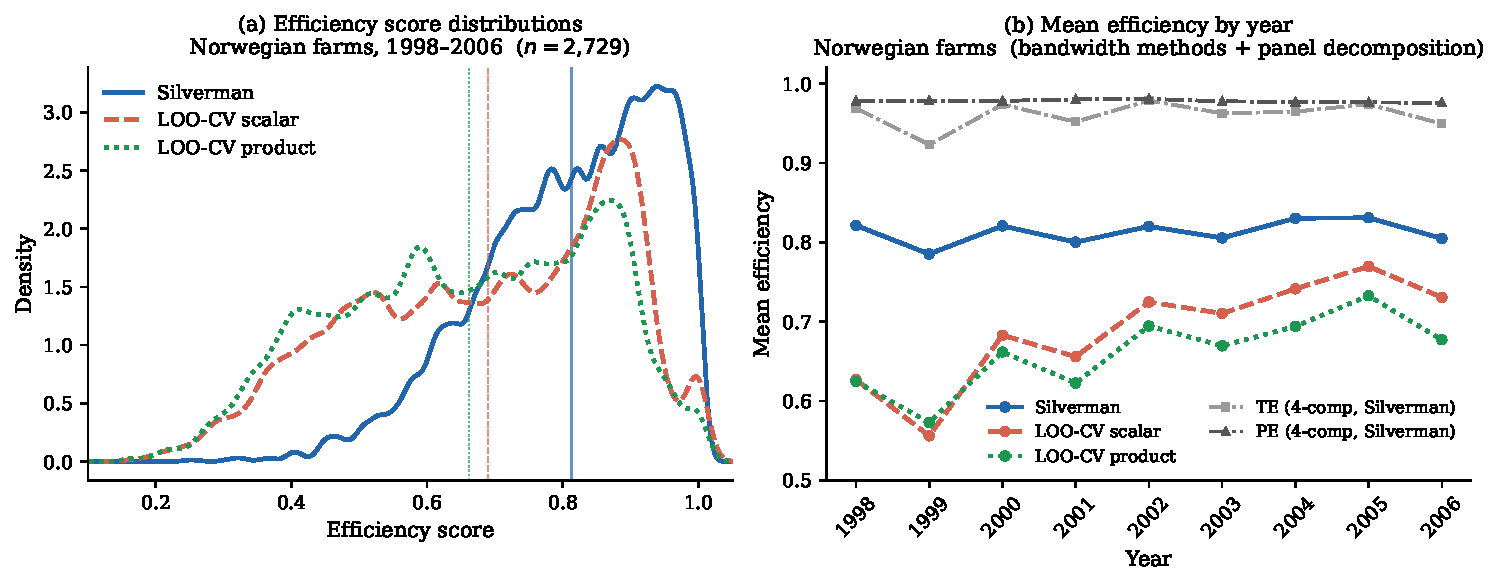
\includegraphics[width=\textwidth]{fig_norway_comparison}
\caption{\label{fig:norway_comparison}%
  Bandwidth sensitivity and panel decomposition, Norwegian agricultural
  panel, 1998--2006 ($n=2{,}729$, 460~farms).
  \emph{Left}: kernel density estimates of cross-sectional efficiency
  scores under Silverman rule, scalar LOO-CV (\code{loocv\_scalar}),
  and per-dimension product-kernel LOO-CV (\code{loocv}).
  Vertical lines mark the respective means.
  \emph{Right}: annual means of all three cross-sectional estimates
  together with transient efficiency (TE) and persistent efficiency
  (PE) from \code{PanelSW2023} (Silverman bandwidth).
  The stable, high PE series indicates that most measured
  cross-sectional inefficiency is transient rather than structural.}
\end{figure}


%% -- Summary -----------------------------------------------------------------

\section[Summary and discussion]{Summary and Discussion}
\label{sec:summary}

\pkg{sw2023} provides a complete \proglang{Python} implementation of
the nonparametric multiple-output stochastic frontier estimator of
\citet{SimarWilson2023}, validated against their published simulation
results (Table~F.1).  Key contributions beyond the base estimator include
corrected individual bootstrap confidence intervals (evaluated at the
original $Z$ points after refitting on resampled data), pointwise
asymptotic CIs via the delta method, and a wild bootstrap significance
test for inefficiency heterogeneity \citep{PSVKZ2024}.

Among Python packages for nonparametric frontier estimation,
\pkg{pyStoNED} \citep{DaiFangLeeKuosmanen2024} is the closest counterpart:
both packages support multiple outputs and impose no parametric functional
form.  The key distinction is that \pkg{pyStoNED} builds on CNLS, which
enforces global shape constraints (concavity and monotonicity) and delegates
computation to an external QP solver, while \pkg{sw2023} uses LLLS
without shape restrictions, requires no external solver, and provides
a richer statistical inference toolkit rooted in the asymptotic theory
of \citet{SimarWilson2023} and \citet{PSVKZ2024}.
The two packages are therefore complementary: \pkg{pyStoNED} is preferable
when economic theory strongly justifies the shape constraints, while
\pkg{sw2023} is preferable when shape-unrestricted estimation or
bootstrap inference is needed.

Several limitations of the SW(2023) estimator and the present
implementation deserve mention.
First, efficiency scores depend on the choice of direction vector
$\mathbf{d}$, which must be specified prior to estimation; the package
offers mean- and median-based defaults but no formal test for
direction sensitivity.
Second, the nonparametric LLLS estimator suffers from the curse of
dimensionality: the convergence rate is $n^{2/(d+4)}$ with
$d = p+q-1$, so datasets with many inputs and outputs require
substantially larger samples for reliable estimation.
Third, the wrong-skewness problem --- in which the empirical third
moment of the residuals has the incorrect sign --- is resolved by
setting $\hat\sigma_\eta = 0$ (HMS correction), which implies that
no inefficiency is detected for the affected observations; this occurs
in 50.6\% of the Norwegian sample, underscoring the difficulty of
separating noise from inefficiency in moderate-noise environments.
Fourth, unlike CNLS-based approaches, \pkg{sw2023} imposes no shape
constraints on the frontier, so estimated frontiers may violate
economic regularity conditions (monotonicity, concavity) in finite
samples.
Finally, LOO-CV bandwidth selection, while asymptotically optimal,
is computationally demanding --- $O(d \cdot n^2)$ per regression
step --- and may be impractical for very large datasets without
further approximation.

Future work includes: (i)~prediction intervals for individual efficiency
scores following \citet{SimarWilson2010}; (ii)~extension to revenue and
cost distance functions; and (iii)~extending the native \proglang{Stata}
ado-file to the four-component panel model, which currently requires
the \proglang{Python} interface.


%% -- Computational details ---------------------------------------------------

\section*{Computational details}

The results in this paper were obtained using \proglang{Python}~3.10.4
with \pkg{numpy}~2.2.6 \citep{HarrisEtAl2020},
\pkg{scipy}~1.15.3 \citep{VirtanenEtAl2020}, and
\pkg{pandas}~2.3.3 \citep{McKinney2010}.
\proglang{Python} and all packages are available from the
Python Package Index (PyPI) at \url{https://pypi.org/}.
The \pkg{sw2023} package (version~0.3.1, GPL-3.0-or-later) is available at
\url{https://pypi.org/project/sw2023/}.
Source code is publicly available at
\url{https://github.com/renegade68/sw2023} and the replication script
\code{replication.py} is included with the submission materials.


%% -- Acknowledgments ---------------------------------------------------------

\section*{Acknowledgments}

The author thanks Léopold Simar and Paul W.\ Wilson for making their
simulation design publicly available, and the anonymous reviewers for
helpful comments.


%% -- Bibliography -------------------------------------------------------------

\bibliography{sw2023_refs}


\end{document}
